\section{Active learning (Stage 1)}
\label{sec:visualizer:al}

The main goal of stage 1 is to learn the user's interests. This requires the 
system to select (``query'') data (which are $n$ characterizations of $d\choose 
2$ plots in the case of the VS as described in 
Section~\ref{sec:visualizer:scatterplot:features}) for the analyst (the 
``oracle'') to label (classify). This is \textbf{stage 1}. 
The learner may then utilize 
a classification model (discriminant analysis, naive Bayes, decision tree(s), 
logistic regression, etc.) that trains on labeled data to ``learn'' user 
interests. The user's interests are encoded in a classifier (some instance of 
the classification model) that is applied to automatically label the rest of 
the data (For more on the 
semantic differences between ``classification model'' and ``classifier'' in 
this body of work, see Figure~\ref{fig:visualizer:al:tree}). This is 
\textbf{stage 2} (Section~\ref{sec:visualizer:plotgeneration}). 
As such, it is important to make the process as efficient as possible to avoid 
redundancy for the end user. There are various methods that may be used for 
querying in stage 1~\cite{dasgupta2011}:

\tablespacing
\begin{itemize}
	\item \textbf{Supervised learner}: This learner queries a single, random 
	subset of all unlabeled data. It ignores the rest of the data when refining 
	the classifier
	\item \textbf{Semisupervised learner}: Similar to a supervised learner, a 
	semisupervised learner queries a single, random subset of all 
	unlabeled data but proceeds to utilize the remaining unlabeled data to 
	better inform the final classifier
	\item \textbf{Active learner}: An active learner selects its queries in a 
	non-random, intelligent manner to reduce the hypothesis space $\mathcal{H}$ 
	of all possible classifiers that may explain the data.
\end{itemize}
\bodyspacing

It has been 
shown that when a learning algorithm is allowed to choose its next query, it 
performs better with less training; as such, we choose to utilize active 
learning to select the plots to be queried by the oracle in stage 
1~\cite{settles2010}. Chapter~\ref{ch:al} goes into detail on different active 
learning methodologies as this section is primarily focused on its role in the 
system.

\begin{figure}[htb]
	\begin{center}
		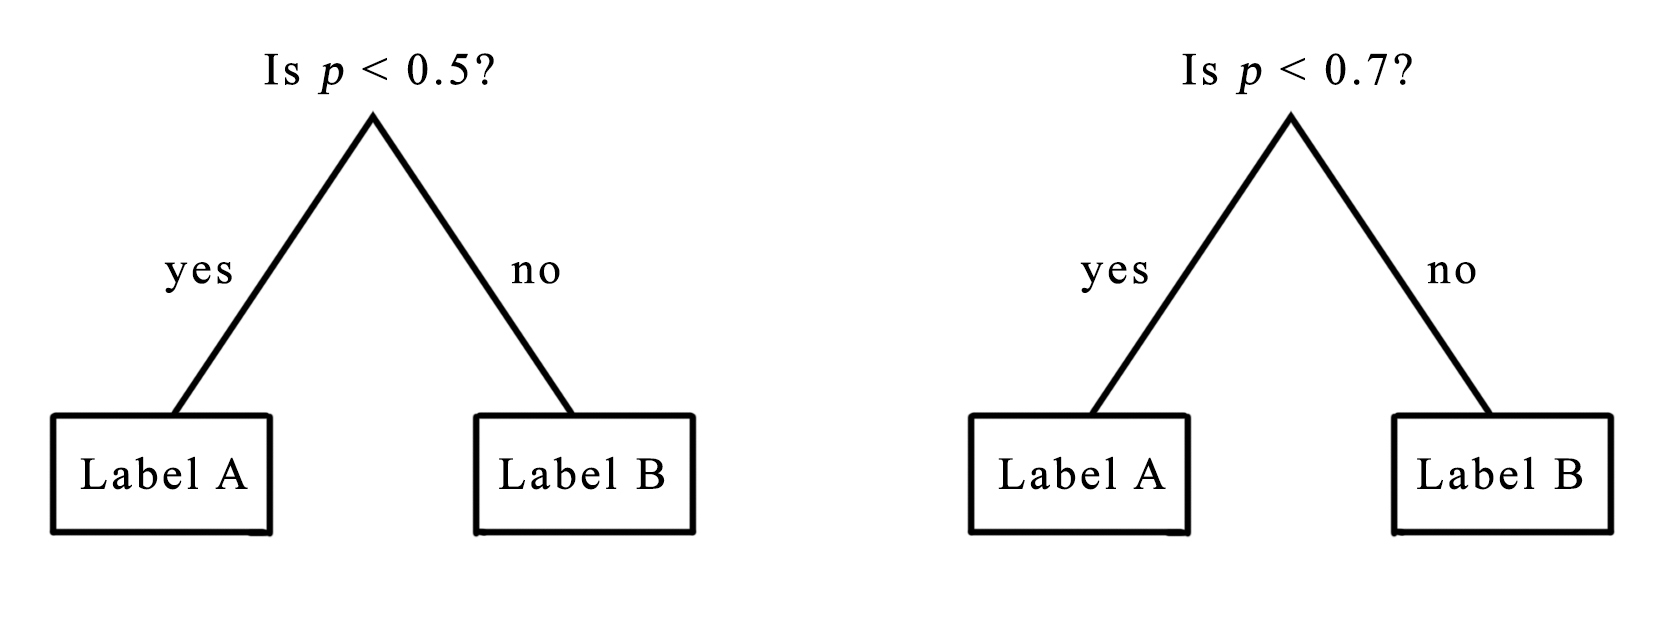
\includegraphics[width=0.75\linewidth]{ch-visualizer/figures/tree}
		\caption[Classifiers and classification models]{Although both figures 
		on the left and right are slightly different classifiers, they 
		are both instances of (extremely simple) decision trees, a type of 
		classification model. Other models include discriminant analysis, naive 
		Bayes, random forest, logistic regression, etc. 
		See Section~\ref{sec:visualizer:plotgeneration:tree} for more details 
		on trees.}
		\label{fig:visualizer:al:tree}
	\end{center}
\end{figure}

\subsection{Initialization of active learner}
\label{sec:visualizer:al:initialization}

It is problematic to start from scratch; how does the system determine
the best first point of ambiguity when it knows nothing (the hypothesis space is
everything)? A classic method is to simply select $k$ random data instances for 
the user to label. As initialization is not the focus of this work, the VS 
currently utilizes this methodology.

Alternatively, we can exploit the fact that the
user is already providing a numerical model that they believe to be a good
representation of the data which they would like the visualization system to
check visually. Given this data, the system may build a classifier that utilizes
the various properties of the plots to determine whether one is interesting or
uninteresting. Doing so greatly narrows the hypothesis space and makes it easier
to determine points of ambiguity. However, to reconcile with the fact that the
user wishes to check the numerical model and may not necessarily believe it is a
good representation of fit, the learner must check whether the initial 
classifier is a proper fit (This may be achieved with line-up tests, which are 
described briefly in Section ~\ref{sec:futurework:lineup}). As the user then 
proceeds to label various conditional plots (queried by the active learner) as 
``interesting'' or ``not interesting,'' the learner better understands the
user’s interest, and the final classifier continues to evolve and improve.

\subsection{Query selection}
\label{sec:visualizer:al:tree}

Post-initialization, the active learner cleverly queries vital plots so that 
the system can best learn the user’s interests. The system first determines 
which features it is uncertain about classifying and then returns a plot 
matching those characteristics to the user. This allows the system to utilize 
its classification model of choice to build a better classifier more 
efficiently. \textbf{
	It is important to distinguish between the active learner, which 
	selects the next queries from the pool of unlabeled data and \textit{may 
		use 
		its own classification model(s) to aid in query selection}, and the VS, 
	which 
	uses a \textit{single classification model} to fit both the initialization 
	and actively selected queries in order to build a model to classify the 
	user's 
	interests and label the remaining plots in Stage 2 }
(Section~\ref{sec:visualizer:plotgeneration}). 
Various active learning (selection) algorithms include uncertainty sampling, 
query by committee, query by bagging, and min-max clustering, all of which are 
described more thoroughly in Chapter~\ref{ch:al}.